\section{태스크}
태스크는 간단하게 Activity 작업 묶음 단위라고 보면 된다. 사진 리스트를 보고(PictureListActivity), 사진 상세를 보고(PictureDetailActivity), 사진을 올리려고 카메라를 실행시킨다(Camera 앱).
하나의 앱이 하나의 태스크가 아니라는 것을 염두에 두자. 물론 하나의 앱만 사용하면서, 그 안에 여러 개의 태스크를 가질 수도 있다.(보통은 안 그렇지만)\\
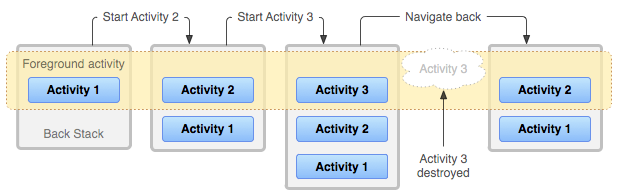
\includegraphics[scale=0.6]{diagram_backstack}

Activity는 스택에 차례대로 쌓인다.(Back Stack으로 불린다.) 스택은 말 그대로 First In, Last Out 방식으로 쌓이고 사라진다. 스택 구조라서 넣거나 빼기만 할 수 있고 순서를 바꿀 수 없다고 개발자 가이드에 있지만 꼭 그렇진 않다. Intent.FLAG\_ACTIVITY\_REORDER\_TO\_FRONT 플래그를 사용하면 순서를 조정할 수 있다.\\

단순하게 startActivity()를 실행해서 스택에 추가하고, Back 키로 제거해가면 아무 일도 없지만, 실제 앱에서는 다양한 경로의 Activity 접근이 이루어지기 때문에 내비게이션이 꼬이는 경우가 많이 생긴다. 이 때문에 태스크 관리가 필요하다.

예를 들어보자. 
\begin{enumerate}
\item 캘린더 앱은 기본 달력 화면(A)에서 일정상세 화면(B)으로 가고 다시 일정수정 화면(C)으로 이동한다. 그러다가 Home 키를 눌러서 태스크를 백그라운드로 보낸다. 
그런데 홈 스크린 화면에 일정목록 App Widget이 있어서 특정한 일정으로 이동할 수 있다. 그렇다면 이 특정한 일정 보기 화면은 앞에 있던 A, B, C 위에 B를 추가하면 될까? 아니면 C를 스택에서 없애고, B를 다시 로딩하게 할까?
\item 사진 공유앱에서 사진 목록 화면(A)에서 사진등록자의 프로필 이미지를 클릭하면 등록자의 프로필을 포함한 동록자의 사진 목록 화면(B)로 이동한다. B 화면의 사진들에는 ``좋아요''를 한 사용자 이미지들이 있는데 이 이미지를 클릭하면 그 사용자의 사진 목록 화면 B'으로 이동한다. 계속 반복해서 사용자의 사진 목록 화면이 쌓일 수도 있고, 아니면 같은 화면에서 화면만 갱신할 수도 있다. 어느 쪽이 원하는 방식일까?
\end{enumerate}

각 앱에서 원하는 내비게이션 방식이 있는데, 태스크의 동작 방식을 이해하지 못한다면 사용자가 보고자 하는 화면이 아닌 엉뚱한 화면을 접하는 경우가 생긴다. 물론 이해가 간단하지 않고 많은 시행착오가 우리 앞에 기다리고 있다.

\subsection{태스크 상태}
태스크는 화면에 포커스되어 있는 포그라운드 상태와, 화면에 보이지 않는 백그라운드 상태가 있다. 포그라운드에 있는 것은 Home 키를 통해서 언제든 백그라운드로 이동할 수 있다.
백그라운드에 있는 것도 언제든 포그라운드로 이동할 수 있다. 앱 아이콘이나 Shortcut, App Widget, Notification을 통해 새로운 포그라운드 태스크가 될 수도 있다. Home 화면에 나와있는 경우는 Home 화면이 포그라운드 태스크이다.\\

백그라운드 상태를 변경할 수 있는 메서드는 Activity에 moveTaskToBack(boolean nonRoot) 메서드가 있다. nonRoot에 true가 들어가면 어느 위치에서건 백그라운드로 이동할 수 있고, false인 경우에는 태스크 루트일 때만 가능하다. 
메서드 시그너처를 보고서 파라미터의 용도를 볼 때마다 헷갈리는 걸 보면 잘 만든 메서드는 아닌 듯 하다. 메서드 시그너처를 moveTaskToBack(boolean onlyRoot) 이런 식으로 바꾸면 좀 낫지 않을까. \\

이제 반대로 백그라운드에서 포그라운드로 상태를 변경하는 메서드는 있을까? 
Activity가 보이지 않는 백그라운드 상태이기 때문에 Activity의 메서드로는 안 된다.
바로 ActivityManager에서 
List$<$ActivityManager.Running\-TaskInfo$>$ getRunningTasks(int maxNum) 메서드를 통해서 가장 최근의 maxNum 개를 가져오고 moveTaskToFront(int taskId, int flags) 메서드에 RunningTaskInfo.id를 taskId에 전달하면 된다.\footnote{관련해서 \url{http://bonjwakim.tistory.com/15}를 참고하자.}
% 권한 필요

\subsection{태스크 확인}
눈으로 화면이 바뀌는 것을 기준으로 테스트하면 태스크가 정상적으로 동작하는지 확인하기 어렵다. Back 키로 이전 화면으로 돌아가면 잘 남아있다고 동일한 태스크라고 확신할 수 없다.
예를 들어, 앱에서 startActivity()를 실행해서 브라우저를 열었다면 앱과 브라우저는 한 묶음 같아 보인다. 그런데 과연 동일한 태스크일까? 그렇지 않다. 브라우저는 singeTask lanuchMode로 되어 있어서 별도의 태스크로 되어 있다.\\

shell에서 dumpsys를 활용해서 태스크를 확인하면서 각 상황을 이해하도록 하자.
adb shell dumpsys activity activities를 실행하거나, adb shell하고서 shell 안에서 dumpsys activity activities를 실행하면 된다. 마지막 옵션인 activities는 줄여서 a로 써도 된다.\\

dumpsys 내용이 많은 경우 한번에 확인하기 어려워서 리다이렉션을 통해 파일로 저장하는 것을 권장한다. adb shell dumpsys activity a  $>$ tasks.txt 와 같이 사용한다. adb shell 안에서도 dumpsys를 할 수 있지만 shell 내에서는 리다이렉션이 되지 않는다.\\

그래도 워낙 내용이 많긴 하다. 해당 앱 관련 내용만 볼 때는 grep 명령어를 활용하자. dumpsys activity a | grep com.example.android.supportv4 이런 식으로 하면 관련 라인만 볼 수 있다. 필자의 경우는 grep을 통해서 일부만 보면 필요한 정보를 빠뜨릴 수 있지 않나 생각해서 잘 안 쓰는 편이었는데, dumpsys 내용에 패키지명이 계속해서 들어가기 때문에 grep을 통해서 보는 편이 낫다.\\

아래는 adb shell dumpsys activity a를 실행한 결과이다. 참고로 안드로이드 버전마다 dumpsys 결과는 다를 수 있다. \ref{sec:dumpsys} 절에서 dumpsys 명령어를 상세히 보기로 한다.
\lstset{basicstyle=\fontfamily{mono}\selectfont\scriptsize}
\begin{lstlisting}[frame=single]
ACTIVITY MANAGER ACTIVITIES (dumpsys activity activities)
  Main stack:
  * TaskRecord{43495e10 #132 A com.example.android.supportv4 U 0}
    numActivities=3 rootWasReset=false userId=0
    affinity=com.example.android.supportv4
    intent={act=android.intent.action.MAIN cat=[android.intent.category.LAUNCHER] 
    flg=0x10000000 cmp=com.example.android.supportv4/.Support4Demos}
    realActivity=com.example.android.supportv4/.Support4Demos
    askedCompatMode=false
    lastThumbnail=android.graphics.Bitmap@42fcd710 lastDescription=null
    lastActiveTime=123128734 (inactive for 36s)
    * Hist #36: ActivityRecord{432c0720 com.example.android.supportv4/.app.FragmentTabs}
        packageName=com.example.android.supportv4 processName=com.example.android.supportv4
        launchedFromUid=10194 userId=0
        app=ProcessRecord{42c11768 18847:com.example.android.supportv4/u0a194}
        Intent { cmp=com.example.android.supportv4/.app.FragmentTabs }
        frontOfTask=false task=TaskRecord{43495e10 #132 A com.example.android.supportv4 U 0}
        taskAffinity=com.example.android.supportv4
        realActivity=com.example.android.supportv4/.app.FragmentTabs
        baseDir=/data/app/com.example.android.supportv4-2.apk
        dataDir=/data/data/com.example.android.supportv4
        stateNotNeeded=false componentSpecified=true isHomeActivity=false
        compat={320dpi always-compat} labelRes=0x7f07002a icon=0x7f020001 theme=0x0
        config={1.15 450mcc5mnc ko_KR sw384dp w384dp h615dp nrml long port finger 
        -keyb/v/h -nav/h s.110fontTypeIndex}
        launchFailed=false haveState=true icicle=Bundle[mParcelledData.dataSize=3540]
        state=STOPPED stopped=true delayedResume=false finishing=false
        keysPaused=false inHistory=true visible=true sleeping=true idle=true
        fullscreen=true noDisplay=false immersive=false launchMode=0
        frozenBeforeDestroy=false thumbnailNeeded=false forceNewConfig=false
        thumbHolder=TaskRecord{43495e10 #132 A com.example.android.supportv4 U 0}
        waitingVisible=false nowVisible=true lastVisibleTime=-1m8s283ms
    * Hist #35: ActivityRecord{42d3e318 com.example.android.supportv4/.Support4Demos}
        packageName=com.example.android.supportv4 processName=com.example.android.supportv4
        launchedFromUid=10194 userId=0
        app=ProcessRecord{42c11768 18847:com.example.android.supportv4/u0a194}
        Intent { cmp=com.example.android.supportv4/.Support4Demos (has extras) }
        frontOfTask=false task=TaskRecord{43495e10 #132 A com.example.android.supportv4 U 0}
        taskAffinity=com.example.android.supportv4
        realActivity=com.example.android.supportv4/.Support4Demos
        baseDir=/data/app/com.example.android.supportv4-2.apk
        dataDir=/data/data/com.example.android.supportv4
        stateNotNeeded=false componentSpecified=true isHomeActivity=false
        compat={320dpi always-compat} labelRes=0x7f070000 icon=0x7f020001 theme=0x0
        config={1.15 450mcc5mnc ko_KR sw384dp w384dp h615dp nrml long port finger 
        -keyb/v/h -nav/h s.110fontTypeIndex}
        launchFailed=false haveState=true icicle=Bundle[mParcelledData.dataSize=1284]
        state=STOPPED stopped=true delayedResume=false finishing=false
        keysPaused=false inHistory=true visible=false sleeping=true idle=true
        fullscreen=true noDisplay=false immersive=false launchMode=0
        frozenBeforeDestroy=false thumbnailNeeded=false forceNewConfig=false
        thumbHolder=TaskRecord{43495e10 #132 A com.example.android.supportv4 U 0}
        waitingVisible=false nowVisible=false lastVisibleTime=-1m13s34ms
    * Hist #34: ActivityRecord{42c07700 com.example.android.supportv4/.Support4Demos}
        packageName=com.example.android.supportv4 processName=com.example.android.supportv4
        launchedFromUid=2000 userId=0
        app=ProcessRecord{42c11768 18847:com.example.android.supportv4/u0a194}
        Intent { act=android.intent.action.MAIN cat=[android.intent.category.LAUNCHER] 
        flg=0x10000000 cmp=com.example.android.supportv4/.Support4Demos }
        frontOfTask=true task=TaskRecord{43495e10 #132 A com.example.android.supportv4 U 0}
        taskAffinity=com.example.android.supportv4
        realActivity=com.example.android.supportv4/.Support4Demos
        baseDir=/data/app/com.example.android.supportv4-2.apk
        dataDir=/data/data/com.example.android.supportv4
        stateNotNeeded=false componentSpecified=true isHomeActivity=false
        compat={320dpi always-compat} labelRes=0x7f070000 icon=0x7f020001 theme=0x0
        config={1.15 450mcc5mnc ko_KR sw384dp w384dp h615dp nrml long port finger 
        -keyb/v/h -nav/h s.110fontTypeIndex}
        launchFailed=false haveState=true icicle=Bundle[mParcelledData.dataSize=1284]
        state=STOPPED stopped=true delayedResume=false finishing=false
        keysPaused=false inHistory=true visible=false sleeping=true idle=true
        fullscreen=true noDisplay=false immersive=false launchMode=0
        frozenBeforeDestroy=false thumbnailNeeded=false forceNewConfig=false
        thumbHolder=TaskRecord{43495e10 #132 A com.example.android.supportv4 U 0}
        waitingVisible=false nowVisible=false lastVisibleTime=-1m21s22ms
  * TaskRecord{43294328 #131 A com.example.android.apis U 0}
        ......
        
  Running activities (most recent first): // (1)
    TaskRecord{43495e10 #132 A com.example.android.supportv4 U 0}
      Run #12: ActivityRecord{432c0720 com.example.android.supportv4/.app.FragmentTabs}
      Run #11: ActivityRecord{42d3e318 com.example.android.supportv4/.Support4Demos}
      Run #10: ActivityRecord{42c07700 com.example.android.supportv4/.Support4Demos}
    TaskRecord{43294328 #131 A com.example.android.apis U 0}
      Run #9: ActivityRecord{42f55e10 com.example.android.apis/.app.FinishAffinity}
	....
 
  mResumedActivity: null
  mFocusedActivity: ActivityRecord{432c0720 com.example.android.supportv4/.app.FragmentTabs} // (2)
  mLastPausedActivity: ActivityRecord{432c0720 com.example.android.supportv4/.app.FragmentTabs}
  mSleepTimeout: false
  mDismissKeyguardOnNextActivity: false

  Recent tasks: // (3)
  * Recent #0: TaskRecord{43495e10 #132 A com.example.android.supportv4 U 0}
    numActivities=3 rootWasReset=false userId=0
    affinity=com.example.android.supportv4
    intent={act=android.intent.action.MAIN cat=[android.intent.category.LAUNCHER] 
    flg=0x10000000 cmp=com.example.android.supportv4/.Support4Demos}
    realActivity=com.example.android.supportv4/.Support4Demos
    askedCompatMode=false
    lastThumbnail=android.graphics.Bitmap@42fcd710 lastDescription=null
    lastActiveTime=123128734 (inactive for 37s)
  * Recent #1: TaskRecord{43294328 #131 A com.example.android.apis U 0}
    numActivities=4 rootWasReset=false userId=0
    affinity=com.example.android.apis
    intent={act=android.intent.action.MAIN cat=[android.intent.category.LAUNCHER] 
    flg=0x10000000 cmp=com.example.android.apis/.ApiDemos}
    realActivity=com.example.android.apis/.ApiDemos
    askedCompatMode=false
    lastThumbnail=android.graphics.Bitmap@42ec86d0 lastDescription=null
    lastActiveTime=123083178 (inactive for 82s)
.....

  mCurTask: 132          
\end{lstlisting}
\lstset{basicstyle=\ttfamily\small}
\begin{itemize}
\item 태스크는 최신 것이 먼저 위쪽에 나타난다.
\item TaskRecord 섹션에서는 numActivities와 그 안의 Hist 섹션을 통해 스택을 들여다볼 수 있다. 다양한 설정 데이터도 보여준다. ProcessRecord에는 프로세스명(패키지명) 앞뒤로 프로세스의 PID와 USER ID도 보여준다.(shell에서 ps 명령어로 확인해보자.)
TaskRecord에는 app=null로 나오고, state=DESTROYED로 있는 것도 볼 수 있는데, 프로세스가 종료된 것이다. 아래 쪽으로 가면 하루나 이틀 지난 것까지도 나온다. 말 그대로 히스토리이다. 
\item 79 라인(1)에 Running activities 섹션은 스택의 간략한 내용으로 나온다.
\item 94 라인(3)에 RecentTasks 섹션도 내용이 반복되지만, 태스크의 간략한 개요가 나온다.(numActivities 등)
\item 89 라인(2)에 화면에 포커스되어 있는 Activity가 나온다.
\item 마지막 라인에 현재 포그라운드에 있는 태스크를 보여준다. 홈 화면도 하나의 태스크이기 때문에 홈 화면으로 나와있다면 Launcher가 현재 태스크로 보인다.\footnote{시점에 따라 백그라운드의 태스크 번호를 보여주기도 한다. 이 번호는 참고 데이터 정도로만 생각하자.}
\end{itemize}
% 케이스를 좀 더 확인할 수 있을까?
dumpsys 명령어는 개발 중에 현재 포커스된 Activity가 어떤 것인지 확인하는 데도 유용하다.
테스트하면서 여러 Activity를 이동하는데, Activity가 많으면 현재 어느 Activity에 있는지 찾아가는 게 간단치 않다.
이 명령어를 몰랐을 때는 시작 Activity부터 로직을 따라가서 현재 Activity를 찾기도 했다. ApiDemos에서 기능을 테스트해보다 관련 Activity를 찾아서 디렉토리를 뒤져본 기억들은 안드로이드 앱 개발자라면 가지고 있을 것이다.

\subsection{taskAffinity}
Activity에서 startActivity()를 실행하는 게 많지만, 알람 같은 경우 BroadcastReceiver에서 startActivity()를 실행하는 것이 일반적이고 Service 실행 중에 Activity를 시작하는 상황도 있다. Application에서는 드물지만 이벤트를 항상 받기 위해서 Application에 BroacastReceiver를 등록하고 여기서 startActivity()를 실행하는 경우가 있다.
그런데 Activity가 아닌 곳에서 startActivity()를 실행하는 경우에는 앱이 포그라운드에 있을 수도 있지만, 기본적으로 백그라운드에서 실행한다고 가정해야만 한다. Activity 외에 다른 컴포넌트에서 startActivity를 실행하면 아래와 같은 에러를 만날 때가 있다.
\begin{lstlisting}[frame=single]
09-07 08:49:32.314: E/AndroidRuntime(482): Caused by: android.util.AndroidRuntimeException: 
Calling startActivity() from outside of an Activity  context requires 
the FLAG_ACTIVITY_NEW_TASK flag. Is this really what you want?
\end{lstlisting}

에러 메시지에 있는 대로 Intent.FLAG\_ACTIVITY\_NEW\_TASK 플래그를 포함해야 한다.
\begin{lstlisting}[frame=single]
Intent intent = new Intent(context, ScheduleViewerActivity.class);
intent.putExtra(SheduleViewerActivity.CALEDAR_ID, 20);
intent.setFlags(Intent.FLAG_ACTIVITY_NEW_TASK);
context.startActivity(intent);
\end{lstlisting}

이미 해당 앱이 태스크 목록에 이미 있는 경우는 어떨까? 태스크가 새로 하나 생성되면서 ScheduleViewerActivity가 뜨는가 하면 그렇지 않다. 바로 taskAffinity가 동일한 게 있다면 이 태스크 위에 뜨게 된다. 
taskAffinity는 AndroidManifest.xml의 Activity 선언에 android:taskAffinity에 지정할 수 있고 속성이 없다면 디폴트 값은 패키지명이다.
결국 taskAffinity 속성을 선언하지 않은 것끼리는 FLAG\_ACTIVITY\_NEW\_TASK 속성을 쓰더라도 같은 태스크에 있게 된다.
taskAffinity는 보통은 안 쓰는 속성이지만, 내부적으로 이런 게 일어나고 있어서, FLAG\_ACTIVITY\_NEW\_TASK를 써도 새로운 태스크가 생기지 않는 것이다.
별도로 속성을 줄 때는 android:taskAffinity=``:alarm'' 식으로 프로세스 분리할 때처럼 :(clone) 뒤에 구분자를 적는 것을 권장한다.\footnote{com.example.android.lifecycle.another 또는 :another와 같은 형식이 모두 가능하지만  another처럼 단순한 이름을 쓰는 것은 허용되지 않는다.}\\

Activity 선언에 taskAffinity 속성을 따로 주는 경우를 알아보자. 다른 화면들과 독립적인 알람 화면 같은 경우가 그렇다. 
알람 앱에 알람 리스트 화면(AlarmClock), 알람 설정 화면(AlarmSettings), 알람 화면(AlarmAlert)과 같이 세 개의 화면이 있다고 하자. 
만일 AlarmAlert 화면에 android:taskAffinity 속성이 따로 없다면 어떻게 될까?
일정 시간이 되어 알람이 떴는데 그 순간에 알람 앱의 태스크가 포그라운드나 백그라운드에 이미 있을 수 있다. 
그러면 AlarmAlert 화면이 뜰 때 백그라운드에 있다면 함께 포그라운드로 올라와서 맨 위에 AlarmAlert 화면이 있을 것이고, 포그라운드에 이미 있었다면 AlarmAlert 화면이 그 위에 추가되어서 포커스될 것이다.
백그라운드에 있던 화면이 딸려 올라오는 것도 동작이 이상하다. 결국 이미 포그라운드에 있던 것처럼 동작하게 된다. Back 키를 누르니 방금 전까지 보이지 않았던 알람 설정 화면이 뜨는 것이다.\\

이런 케이스를 막기 위해서 AlarmAlert의 taskAffinity를 다르게 세팅하면, FLAG\_ACTIVITY\_NEW\_TASK Flags를 추가했을 때 새로운 태스크로 뜨게 되므로 딸려 올라오는 일이 없어진다. 이렇게 되면 태스크가 각각이 되어서 한 앱에서 2개의 태스크를 사용하게 된다.
Home 키를 길러 눌러서 최근 앱 목록을 보면 2개가 떠있는 것을 볼 수 있다. AlermAlert 화면이 최근 앱 목록으로 나오는 것을 방지하기 위해서 AndroidManifest.xml의 AlarmAlert 선언에 android:excludeFromRecents=``true''를 추가하면 알람 기능의 기본 형태를 갖추게 된다.


%https://groups.google.com/forum/#!topic/android-developers/wKwnV1k_96A

\subsection{태스크 속성 부여}
Activity에 태스크 속성을 부여하는 방법에는 2가지가 있다. 속성을 아예 부여하지 않고서 개발할 수 있다면 행복하겠지만, 사용하다 보면 효율적이지 않은 부분이 생긴다.
디폴트는 Activity가 인스턴스가 매번 새로 생성돼서 쌓이는 형태이다.\\
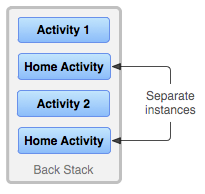
\includegraphics[scale=0.7]{diagram_multiple_instances}\\
속성을 부여하는 2가지 방법은 하나는 불려지는 쪽(Callee )에서 `나를 이런 식으로 취급해줘(존재할거야)'가 있고, 또 하나는 부르는 쪽(Caller)에서 `널 이렇게 다뤄주겠어'하는 것이다. 그리고 2가지 방법의 조합도 있다.
복잡하게 생각할 건 없다. 테스트하면서 원하는 내비게이션 형태를 만드는 과정이 조금 어려울 뿐이다.
아래 설명을 위해서 \url{http://developer.android.com/intl/ko/training/basics/activity-lifecycle/pausing.html}에 있는 ActivityLifecycle.zip을 다운로드하고 변경하면서 테스트해 보자. 
이 샘플에는 ActivityA, ActivityB, ActivityC, DialogActivity(다이얼로그 테마)까지 4개의 Activity가 있다.

\paragraph{Callee 속성 부여는 AndroidManifest.xml의 Activity 선언에 android:launchMode로 한다.}
launchMode에는 standard, singleTop, singleTask, singleInstance 네 가지가 있다. standard와 singleTop은 여러 개의 인스턴스가 존재할 수 있고, singleTask와 singleInstance는 하나의 인스턴스만 존재하다. launchMode 각각을 살펴보자. 설명에서 topActivity(스택의 맨 위)나 baseActivity(스택의 맨 하단)는  ActivityManager.RunningTaskInfo 클래스의 필드명을 그대로 사용했다.
\begin{itemize}
\item standard: 태스크의 topActivity에 매번 새로운 Activity 인스턴스를 생성해서 Intent를 전달한다. Activity의 onCreate() 메서드부터 getIntent() 메서드를 사용할 수 있다.
\item singleTop: 호출하고자 하는 Activity가 이미 topActivity에 있다면 새로 생성하지 않고, onNewIntent() 메서드로 Intent를 전달한다. topActivity에 없을 때는 standard와 동일하게 새로 생성한다.
\item singleTask: 인스턴스는 하나뿐이다. 별도의 태스크로 Activity 인스턴스가 이미 있다면 새로 생성하지 않고, onNewInent() 메서드로 Intent를 전달한다. 
Activity 인스턴스가 없다면 새로운 태스크의 baseActivity로 생성한다. 스택에는 새로운 Activitity를 추가할 수 있다.\\

ActivityLifecycle 샘플에서 ActivityB로 singleTask로 정하고, ActivityA$\rightarrow$ActivityB$\rightarrow$ActivityC 순으로 호출해보자. 하나의 태스크에 모두 쌓이는 것을 볼 수 있다. 바로 taskAffinity가 동일할 때는 아무 의미가 없다. 새로운 태스크로 ActivityB를 띄우려고 하지만 동일한 taskAffinity가 이미 있다면,  ActivityA 위에 그대로 뜨게 된다. 이 내용에 대해서 명시적으로 언급된 부분은 찾지 못했지만 여러 테스트에서도 동일한 결과를 보여 주었다. 이제 ActivityA$\rightarrow$ActivityB$\rightarrow$ActivityC$\rightarrow$ActivityB 순서로 실행해 보자. ActivityC 위에 ActivityB가 올라가진 않고 ActivityC는 스택에서 제거된다. 결과적으로 ActivityA$\Rightarrow$ActivityB 태스크가 남는다. singleTask launchMode의 효과가 전혀 없는 게 아니다.\\

이번에는 ActivityB의 taskAffinity를 변경하고 테스트해 보자. ActivityA$\rightarrow$ActivityB$\rightarrow$ActivityC 순으로 호출하면 ActivityA, ActivityB$\Rightarrow$ActivityC 2개의 태스크가 남게 되다. 
여기서도 ActivityA$\rightarrow$ActivityB$\rightarrow\newline$ActivityC$\rightarrow$ActivityB 순서로 실행해 보자. 역시 ActivityC가 스택에서 제거되고 결국 ActivityA, ActivityB의 2개의 태스크만 남게 된다.\\

앞서 얘기했듯이 모바일 브라우저의 경우가 singleTask launchMode를 사용한다. 
\begin{comment}
http://developer.android.com/intl/ko/training/basics/activity-lifecycle/pausing.html
%이제는 안 그런다..
Facebook에서 기사 링크를 클릭해보면 브라우저가 뜨는데, 이때 dumpsys를 해보면 별도의 Task로 뜨는 것을 확인할 수 있다.\\
이때 홈 키를 길게 눌러서 최근 앱 목록을 확인해보면 Facebook과 브라우저가 각각 따로 보여진다. 당연히 Task가 별개이기 때문에 Facebook을 다시 로딩하면(Recent Apps든, 아이콘을 통해서든), Facebook 화면이 그대로 뜨게 된다.
\end{comment}

\item singleInstance: singleTask와 마찬가지로 인스턴스가 하나뿐이며, 태스크의 유일한 Activity이기도 하다. 여기서 새로운 Activity를 시작하면 이 태스크가 아닌 다른 태스크에 들어가게 되어, 새 태스크를 만드는 효과가 있다. 새 태스크가 되면 새로운 Activity가 뜨는 사이에 검은 화면이 뜨는 시간이 좀 더 오래 걸리는 것을 볼 수 있다. 체감 성능에 차이가 생기므로, 새 태스크가 되어야 하는 케이스와 그렇지 않아도 되는 케이스를 잘 구분하는 것이 좋다.\\

ActivityB의 launchMode가 singleInstance라고 해보자. ActivityA$\rightarrow$ActivityB$\rightarrow$ActivityC 순서로 호출한다고 해보면 재미있는 현상이 발생한다. B는 당연히 하나의 태스크가 된다. 그런데 ActivityA와 ActivityC는 taskAffinity가 동일하기 때문에(ActivityB도 동일하긴 하지만) 하나의 태스크로 다시 묶인다. ActivityC에서 Back 키를 누르면 ActivityB가 아니라 ActivityA로 이동한다. 다시 Back 키를 눌러야만 ActivityB 화면을 볼 수가 있다. 즉 결과로 ActivityA$\Rightarrow$ActivityC, ActivityB 태스크가 된다.\\

ActivityA$\rightarrow$ActivityB$\rightarrow$DialogActivity 순서로 호출해보자. 
DialogActivity는 다이얼로그 테마 Activity이므로 배경에 다른 Activity가 있게 되는데, ActivityB에서 DialogActivity를 띄웠으므로 배경에 ActivityB가 있을 것 같지만, 결과는 ActivityA 화면을 배경으로 깔게 된다.
% Level11 이하에서 동작 테스트해봐야 한다.(동일하네?) http://developer.android.com/reference/android/support/v4/app/TaskStackBuilder.html 참고하자. Level 10에서도 emulator에서 동일했다.
여기서 알 수 있는 것은 Activity를 띄우고서 내부적으로 태스크 조정을 하는 것이 아니라 태스크 조정을 하고나서 Activity를 띄운다는 것이다.(system\_server 프로세스의 ActivityManagerService에서 태스크를 조정한다.) 당연한 얘기인 것 같지만, 이것을 확실하게 알고 있지 않으면 다이얼로그 테마 Activity의 경우처럼 예상치 못한 결과를 볼 수도 있다.\\

최근 앱 목록을 보면 singleInstance로 되어 있는 Activity는 따로 보이지 않는다. 최근 앱 목록도 taskAffinity 기준이라는 것을 알 수 있다.
ActivityB의 taskAffinity를 바꿔주면 어떨까? 결과적으로 태스크가 분리되는 것은 동일하다. 다만 최근 앱 목록에 2개가 따로 뜨는 것을 볼 수 있다.
\end{itemize}
\begin{comment}
singleTask와 singleInstance는 굳이 비유하자면, singleTask는 무조건 새로운 가문을 만들겠다는 것이고, singleInstance는 혼자뿐인 독고다이라고 생각하면 될 듯 하다. 
\end{comment}
singleTask와 singleInstance launchMode는 특별한 상황에서만 사용한다. 사실 태스크 관련 테스트를 하면 제일 헷갈리는 게 이 부분이다.

\paragraph{Caller 속성 부여는 Intent Flags에 지정한다.}
Intent에는 setFlags(int flags) 메서드와 addFlags(int flags) 메서드가 있다. 여기에 전달되는 값은 Intent 클래스의 int 상수인 FLAG\_ACTIVITY\_XXX 값이고, 비트합($|$)으로 여러 개를 전달할 수 있다. 
Intent Flags에 전달하는 값이 Callee의 lanuchMode와 배치되는 경우에는 Callee의 launchMode가 우선한다.\\

Flags에 전달하는 상수는 꽤 많다. Caller에서 쓸 수 있는 다양한 옵션이 있는데 그 가운데 주요한 것을 얘기해보자.
\begin{itemize}
\item FLAG\_ACTIVITY\_SINGLE\_TOP: singleTop launchMode와 동일한 효과를 갖는다.
\item FLAG\_ACTIVITY\_NEW\_TASK: singleTask launchMode와 동일한 효과를 갖는다.

\item FLAG\_ACTIVITY\_CLEAR\_TOP: launchMode에 동일한 효과를 갖는 건 없다. 스택에서 Callee보다 위에 있는 Activity들을 종료시킨다. 앞에서 얘기한 달력(A), 일정상세(B), 일정수정(C) 화면이 스택상에 있다면, B를 띄울 때 이 플래그를 사용하면 C는 사라지고 B에 원하는 일정을 보여주는 식이다. 보통 FLAG\_ACTIVITY\_SINGLE\_TOP 플래그와 같이 쓰이고, 이때 Callee는 남아있어서 onNewIntent() 메서드에 새로운 Intent가 전달된다. FLAG\_ACTIVITY\_SINGLE\_TOP 플래그를 함께 쓰지 않고 단독으로 쓰이면 Callee는 종료하고서 새로 onCreate()부터 실행된다.
% 단독으로 쓰임: B종료->A종료->A시작->C종료
% 같이 쓰임: B종료->A onNewIntent->C종료
이제 FLAG\_ACTIVITY\_CLEAR\_TOP의 한계도 알고 있어야 한다. ActivityA$\Rightarrow$ActivityB$\Rightarrow$ActivityA$\Rightarrow$ActivityB까지 스택에 있을 때 FLAG\_ACTI\-VITY\_CLEAR\_TOP 플래그를 전달해서 ActivityA를 시작하면 어떻게 될까? 맨 아래에 있는 ActivityA만 남으면 좋겠는데 실제로는 맨 위에 있는 ActivityA 기준으로 ClearTop이 되면서 결과로서 ActivityA$\Rightarrow$ActivityB$\Rightarrow$ActivityA가 스택에 남게 된다. 이를 해결하는 방법으로 다음 절에서 <activity-alias>을 활용하는 것을 살펴볼 것이다. 

\item FLAG\_ACTIVITY\_CLEAR\_TASK: Callee가 시작하기 전에 관련한 스택이 모두 제거되고 Callee는 빈 태스크의 baseActivity가 된다. 이 플래그는 FLAG\_ACTIVITY\_NEW\_TASK와 함께 사용되어야 한다. 앱을 사용하면서 태스크에 여러 Activity를 쌓아놓았지만 로그아웃하고 다른 아이디로 로그인한다면, 이 플래그를 사용해서 Launcher Activity를 새로 시작하는 것이 적절할 것이다.(허니콤부터 사용)
\item FLAG\_ACTIVITY\_REORDER\_TO\_FRONT: 태스크에 Activity가 있으면 그 Activity를 스택의 맨 위로 올린다. 해당 Activity가 스택에 하나밖에 없어야만 하는 경우에 쓸 수 있다.
그런데 여기서 주의할 게 2가지 있다. 
\begin{itemize}
\item FLAG\_ACTIVITY\_CLEAR\_TOP 플래그와 함께 사용하면 옵션이 무시된다. 
\item Caller가 Activity일 때만 정상적으로 REORDER가 동작한다. FLAG\_ACTIVITY\_NEW\_TASK를 함께 플래그에 사용해야 하는 Service, BroadcastReceiver, Application에서는 FLAG\_ACTIVITY\_RE\-ORDER\_TO\_FRONT가 동작하지 않는다.
\end{itemize}
\end{itemize}

\begin{comment}
이를테면 앱에다 Passcode 기능(해당 앱이 Forground로 올라올 때마다 암호 입력 화면을 먼저 띄우는 기능)을 추가했다고 하면, 앱 최초 실행시나 Background에서 Foreground로 올라올 때에 Passcode 입력 화면이 떠야 한다.\\
Passcode 입력 화면 채로 Home 버튼을 이용해서 Background로 보내버리고, 다음에 알림이나 앱 위젯 같은 것에서 그 Task 위로 다른 Activity A를 띄운다고 하자. 이때도 Foreground로 올라왔으므로, Activity A위에 Passcode 입력 화면이 뜨는 게 맞을 것이다. 그렇다면 여기서 정상적인 암호 입력을 하면 Activity A가 보일 것이고, 여기서 Back 버튼을 누른다면? Task상에 있는 또 다른 Passcode 입력 화면이 뜰 것이다.\\
이런 상황에서 Passcode 입력 화면을 띄울 때, FLAG\_ACTIVITY\_REORDER\_TO\_FRONT을 전달해서 기존에 있던 게 있을때 맨 상위로 올리는 동작을 하면, 이런 상황은 해결된다.\\
\end{comment}

Flags를 쓸 때 제일 중요한 규칙은 가능한 최소한의 플래그만 전달하는 것이다.
진행하는 프로젝트에서 setFlags 메서드에 5개의 플래그를 조합해서 전달하는 것을 본 적도 있는데, 잘 따져보니 2개만 전달하면 문제가 없는 것이었다.
어떻게든 운이 좋게 원하는 동작에 걸리면 된다는 생각보다는 의도가 명확해야만 한다. 그래야 내비게이션이 변경되어도 문제없이 대응할 수 있다. Callee의 launchMode 속성과 Caller의 Flags를 적절하게 사용해서 조합해야 하는 것은 물론이다. 
% FLAG\_ACTIVITY\_CLEAR\_TOP과 FLAG\_ACTIVITY\_SINGLE\_TOP을 당연히 조합해야 한다고 봐야 하나?

\section{<activity-alias>}
AndroidManifest.xml에는 activity-alias 엘리먼트가 있어서 Activity의 별명을 지정해서 쓸 수 있다. 그런데 별명이 도대체 어디에 도움이 될까?
\begin{comment}
필자의 경우에 처음으로 activity-alias를 적용해 본 경우를 얘기해보자.
해당 케이스는 이렇다.
\begin{itemize}
\item 상세 화면이고 이 화면으로 진입하는 다양한 패스가 있다.
\item 화면을 앱+앱 하이브리드로 변경하려고 한다. 이때 기존 코드는 거의 쓸모가 없기 때문에 아예 다른 Activity로 만들려고 한다. DetailActivty$\rightarrow$DetailWebActivity
\item 테스트 후에 문제가 많다면 원래 상태로 다시 복구하려고 한다.
\end{itemize}

DetailActivity를 호출하는 쪽을 DetailWebActivity로 한꺼번에 바꿔주는 것도 가능하다. 소스 버전 관리툴이 있기 때문에 원복이나 다른 작업자와 충돌 문제가 웬만큼 커버된다.
\end{comment}
\begin{enumerate}
\item 기존에 있던 Activity가 없어졌을 때 사용할 수 있다.
예를 들어, SplashPage가 맨 처음 뜨는 화면이었는데, SplashPage를 제거하고 바로 MainActivity를 보여기로 했다.
그런데 SplashPage에 대한 링크가 Shortcut과 같이 기존 버전에서 남아있는 경우가 있다.
기존 Shortcut은 이제 MainActivity를 바라보도록 해야 하는데, 이때 쓰는 것이 바로 activity-alias이다.
\begin{lstlisting}[frame=single]
	<activity-alias
    	android:name=".SplashActivity"
        android:targetActivity=".MainActivity">
\end{lstlisting}
android:name에는 반드시 존재하는 클래스명을 넣을 필요는 없다. new Intent(Context packageContext, Class<?> cls)는 결과적으로 new Intent().setComponent(new ComponentName(String pkg, String cls))와 동일하다. 
Shortcut 외에도 PendingIntent.getActivity() 메서드로 알람에 등록되어 링크가 남는 경우도 있다. 대체하는 화면이 존재한다면 activity-alias으로 기존 Activity 이름을 남겨두는 것을 고려하자.
\item 앞 절에서 FLAG\_ACTIVITY\_CLEAR\_TOP의 한계를 얘기했다. 동일한 이름의 Activity가 여러 개 있을 때, 이 Activity를 기준으로 ClearTop을 하면, 일반적인 요구사항은 맨 아래에 있는 것만 남기고 싶지만, 맨 위에 있는 것 기준으로 ClearTop이 된다. 이때 쓸 수 있는 방법이 Activity를 처음 시작할 때(즉 맨 아래 Activity) activity-alias를 사용하는 것이다. 그러면 activity-alias 이름으로  Activity Stack의 맨 아래에 남게 되어서, activity-alias 이름을 기준으로 startActivity()를 실행하면서 FLAG\_ACTIVITY\_CLEAR\_TOP 플래그가 전달되면 원하는 결과를 얻게 된다.
\begin{lstlisting}[frame=single]
	<activity-alias
    	android:name=".FirstActivityA"
        android:targetActivity=".ActivityA">
\end{lstlisting}
\begin{lstlisting}[frame=single]
	Intent intent = new Intent().setComponent(new Component(this, "com.suribada.android.FirstActivityA"));
	intent.setFlags(Intent.FLAG_ACTIVITY_CLEAR_TOP | Intent.FLAG_ACTIVITY_SINGLE_TOP);
	startActivity(intent);
\end{lstlisting}
\end{enumerate} 

activity-alias를 쓰면서 제한사항도 있다.
바로 android:targetActivity에 들어가는 Activity는 이전에 선언되어 있어야 한다. 
activity-alias에는 쓸 수 있는 속성이 많지는 않다. 기본 속성은 android:targetActivity를 그대로 따르고 intent-filter는 별도로 쓸 수 있다.
